\section{Giới thiệu đề tài}
\subsection{Mô tả đề tài}
	\hspace*{0.5cm} MeowSQL Knight là một trò chơi RPG nhập vai, chiến đấu theo lượt theo màn trên hệ điều hành Windows, Linux và MacOS (các thiết bị sử dụng bàn phím và chuột).\\
	\hspace*{0.5cm} Khác với những trò chơi chiến đấu theo lượt thông thường. Người phải chiến đấu với các quái vật bằng các câu truy vấn của ngôn ngữ SQL (Structured Query Language) và đánh bại chúng. Nhân vật chính sẽ được đặt trong một mê cung gồm các khu vực chơi khác nhau và được yêu cầu hoàn thành nhiệm vụ đề ra trong khu vực chơi đó. Nó có thể là tiêu diệt quái vật, mở rương kho báu, hoặc giải các câu đố trong khu vực chơi. Tuy nhiên, để
	điều khiển nhân vật chính, cũng như thao tác với các đối tượng trong màn chơi, người chơi cần sử dụng câu truy vấn của ngôn ngữ SQL để giải các câu đố, chiến đấu với quái vật và hoàn thành màn chơi. Việc chiến đấu với kẻ thù bao gồm thu thập các dữ kiện trong Schema bằng câu \textbf{select} để xác định đúng điểm yếu kẻ thù, sử dụng các câu lệnh \textbf{insert} vào các bảng phù hợp để tương tác với trò chơi, như sử dụng vật phẩm, tấn công quái vật,...  Công việc của người chơi là sử dụng các câu truy vấn để khai thác thông tin từ Schema một cách hiệu quả, đánh bại kẻ thù và hoàn thành màn chơi.
	 
\subsection{Lí do chọn đề tài}

\hspace*{0.5cm}SQL đang trở thành một trong những ngôn ngữ được sử dụng phổ biến nhất hiện nay trong lĩnh vực kỹ thuật dữ liệu. SQL có thể xuất hiện ở bất cứ đâu, trong hệ thống quản lý nhân sự của công ty, hay trong hệ thống dữ liệu phân tích của một công ty về thống kê. Mặc dù SQL có thể đã cũ, đã xuất hiện các Hệ cơ sở dữ liệu không sử dụng SQL, nhưng nó vẫn rất phổ biến. Hầu như tất cả các tên tuổi lớn nhất trong ngành công nghệ đều sử dụng SQL, kể cả trong những công ty như Facebook, Google, và Amazon vẫn sử dụng SQL để truy vấn dữ liệu và thực hiện phân tích. Và không chỉ các công ty công nghệ, các doanh nghiệp lớn nhỏ đều sử dụng SQL trong hệ thống của doanh nghiệp.\\
\begin{figure}[H]
	\centering
	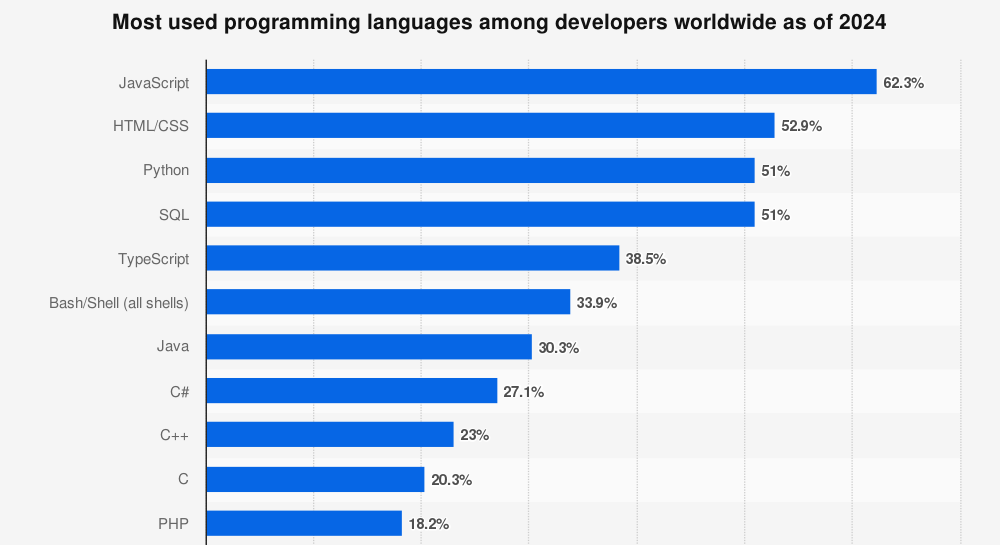
\includegraphics[width=\textwidth]{Images/StatsMostLanguage.png}
	\vspace{0.5cm}
	\caption{Các ngôn ngữ được sử dụng nhiều nhất trong năm 2024. Nguồn: Statista}
\end{figure}


\hspace*{0.5cm}Theo thống kê của trang www.statista.com, trong năm 2024 có đến 51\% Developer được hỏi có sử dụng ngôn ngữ SQL trong công việc. Với độ phổ biến lớn và ổn định qua từng năm, việc học SQL trở thành một phần quan trọng đối với những lập trình viên ở các trình độ khác nhau.\\
Tuy nhiên, việc học một ngôn ngữ declarative như SQL có thể gây nhàm chán, do người học chỉ xoay quanh việc học lý thuyết về các câu truy vấn, các biểu thức trong câu truy vấn, cách này có thể giúp người học nhớ được cấu trúc của cú pháp câu truy vấn, hoặc syntax của biểu thức. Tuy nhiên nếu không nắm rõ công dụng của nó hoặc nắm các vấn đề trong quá trình sử dụng SQL để xử lý dữ liệu, người học có thể quên đi những kiến thức cũ, cũng như dễ mắc cái vấn đề trong quá trình sử dụng ngôn ngữ này. Có một bộ phận người học cũng muốn vừa học ngôn ngữ SQL kết hợp với việc luyện tập tư duy Logic trong việc giải quyết các bài toán từ dễ đến khó thông qua SQL, muốn tìm một công cụ luyện tập lý thú, vừa chơi vừa học.\\

\hspace*{0.5cm} Đây là lý do MeowSQL Knight ra đời. Trò chơi sẽ là nơi để những người đã, đang học, có chỗ để sử dụng SQL hoặc những người muốn tìm hiểu về nó giải trí, rèn luyện tư duy logic.
\subsection{Mục tiêu đề tài}
Thông qua đề tài, nhóm hướng đến xây dựng nhập vai RPG, chiến đấu theo lượt. Thay vì người chơi sử dụng thao thác thông thường để điều khiển nhân vật chính để chiến đấu, người chơi sẽ dùng câu truy vấn SQL để điều khiển nhân vật chính.\\
Trò chơi sẽ như một cầu nối giữa một trò chơi nhập vai đơn thuần với ngôn ngữ truy vấn.
Đây sẽ là nơi mọi người rèn luyện kỹ năng về SQL thông qua các thử thách được đặt ra xuyên suốt trò chơi. Ngoài ra, những người ngoài cũng có thể trải nghiệm trò chơi và nắm được cách hoạt động của các câu truy vấn, cũng như đương đầu với chông gai trong trò chơi. Những người đang học và làm việc với lập trình ngôn ngữ SQL cũng có thể tìm đến trò chơi để giải trí.
\subsection{Đối tượng hướng đến của đề tài}


\hspace*{0.5cm} Các đối tượng mà trò chơi hướng đến có liên quan đến ngôn ngữ truy vấn, sẽ là những người muốn rèn luyện kỹ năng viết câu truy vấn, hoặc những người muốn tìm kiếm một trò chơi giải trí sau những giờ học, làm việc mệt mỏi:
\begin{itemize}
	\item Trò chơi sẽ hướng đến một tập đối tượng tương đối lớn. Họ là những người đã có kiến thức hoặc muốn tìm hiểu về SQL nói riêng, kỹ thuật dữ liệu nói chung. Trò chơi sẽ là một nơi để giải trí đồng thời rèn luyện những kỹ năng về ngôn ngữ truy vấn.
	\item Bản chất của trò chơi là một trò chơi nhập vai mang hơi hướng giải đố, rèn luyện tư duy logic. Những người thích chơi các trò chơi thuộc thể loại này hay những người chơi muốn rèn luyện tư duy cũng có thể chơi được.
\end{itemize}
